\chapter{Periodic Task Scheduling}
\textit{Scheduling} di \textit{tasks} \textbf{periodici} o \textbf{sporadici} (\textbf{aperiodici}). Definiamo un \textbf{task periodico} $\tau_i(C_i, T_i)$ con $C_i$ il \textit{worst case execution time} e $T_i$ il \textbf{periodo} per il quale il task $\tau_i$ deve essere eseguito.
\begin{figure}[h]
    \centering
    \begin{minipage}[t]{0.45\textwidth}
        \centering
        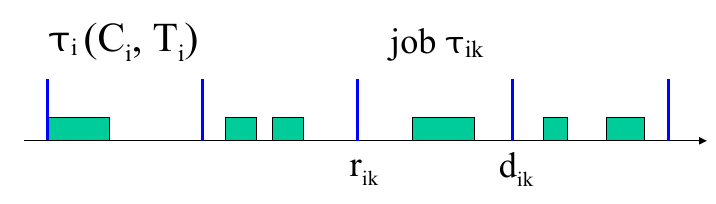
\includegraphics[width=\textwidth]{img/T_aT}
        \caption{\textit{periodic task}}
    \end{minipage}
    \begin{minipage}[t]{0.45\textwidth}
        \centering
        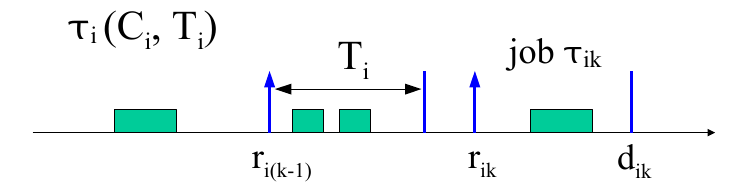
\includegraphics[width=\textwidth]{img/T_aT_1}
        \caption{\textit{sporadic task}}
    \end{minipage}
\end{figure}
\\
Per ogni task periodico, bisogna garantire che:
\begin{itemize}
    \item ogni job $\tau_{ik}$ venga attivato in $r_{ik} = (k - 1) \cdot T_i$.
    \item ogni job $\tau_{ik}$ completi la sua esecuzione entro $d_{ik} = r_{ik} + D_i$.
\end{itemize}
Anche nel caso di \textbf{task aperiodici} possiamo definirli $\tau_i(C_i,T_i)$, in questo caso però $T_i$ non è il periodo nel quale per il quale si ripete il task ma indica il \textit{deelay} minimo di attivazione tra un task $\tau_{ik}$ e un task $\tau_{i(k+1)}$, infatti bisogna garantire per ogni task sporadico che:
\begin{itemize}
    \item ogni job $\tau_{ik}$ viene attivato in un istante $r_{ik} \geq r_{i(k+1)} + T_i$.
    \item ogni job $\tau_{ik}$ completi la sua esecuzione entro una \textit{deadline} relativa $d_{ik} = r_{ik} + D_{ik}$
\end{itemize}

\section{Timeline Scheduling}
È una tipologia di \textit{scheduling offline} è stata utilizzata per anni nei contesti in cui era richiesto un \textit{hard real time} per via della delicatezza delle circostanze di uso (sistemi militari, navigazioni e sistemi di monitoraggio). Può essere chiamato anche \textbf{\textit{cycle executive}} o \textbf{\textit{cyclic scheduling}}. \\
Il funzionamento era tale che l'asse del tempo venisse divisa in intervalli con lunghezza uguale, anche chiamati \textbf{\textit{time slots}}, ogni task viene allocato staticamente in un certo slot e in un certo ordine per venire incontro ai \textit{request rate} desiderati. L'esecuzione per ogni slot viene attivato tramite un \textbf{\textit{timer}}. Consideriamo un task set $\mathcal{T} = \{\tau_1, \tau_2, ..., \tau_k\}$ e che $\forall \tau_i \in \mathcal{T} \; \exists (C_i, T_i)$, in questo caso $T_i \equiv D_i$ ovvero che il periodo del task corrisponde con la sua \textit{deadline} assoluta. Definiremo:
\begin{itemize}
    \item il \textbf{\textit{minor cycle}} come $\Delta = gcd(T_i, T_j) \; \forall T_i, T_j \in \mathcal{T}, \; i \neq j$
    \item il \textbf{\textit{major cycle}} come $\mathbf{T} = lcm(T_i, T_j) \; \forall T_i, T_j \in \mathcal{T}, \; i \neq j$
    \begin{itemize}
        \item nel caso in cui ci siano task sporadici come andiamo a valorizzare il \textit{major cycle}
    \end{itemize}
\end{itemize}
\begin{figure}[h]
    \centering
    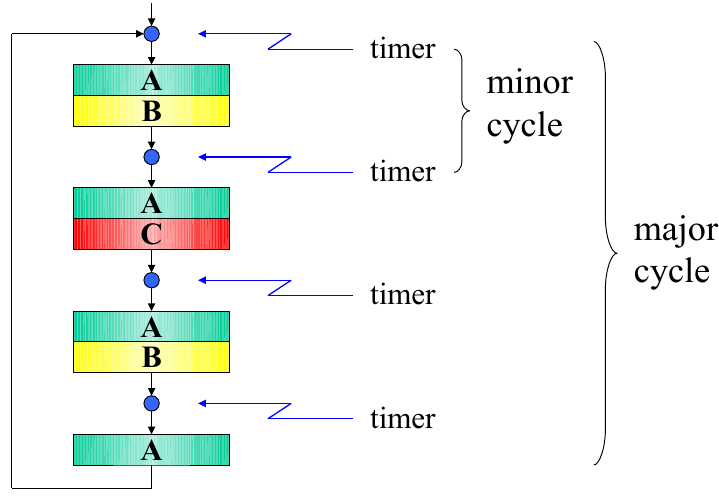
\includegraphics[width=0.5\textwidth]{img/ts}
\end{figure}
\begin{tabular}{ p{7.25cm} | p{7.25cm} }
    \textcolor{green}{\textbf{Vantaggi}} & \textcolor{red}{\textbf{Svantaggi}} \\
    \textbf{-} implementazione semplice (non viene richiesto alcun sistema operativo \textit{real-time}) &  \textbf{-} non è robusto contro \textit{overload} del sistema \\
    \textbf{-} ogni procedura condivide un \textit{address space} comune & \textbf{-} nel caso di aggiunta di un nuovo task è molto difficile l'espansione dello \textit{scheduler} \\
    \textbf{-} basso \textit{overhead} a tempo di esecuzione & \textbf{-} non è facile gestire task aperiodici \\
    \textbf{-} permette di controllare i \textit{jitter} & \textbf{-} tutti i processi devono avere periodo multiplo del \textit{minor cycle} \\
     & \textbf{-} è difficile includere processi con un periodo lungo \\
     & \textbf{-} difficile da costruire e da mantenere \\
     & \textbf{-} tutti i processi con un \textit{WCET} variabile devono essere \textit{splittati} in procedure con lunghezza fissa. (il determinismo non è richiesto, ma la predicibilità si) \\
\end{tabular}
\\ \newline
Durante un \textbf{\textit{overload}} si possono ``considerare'' due vie: la prima è quella di lasciar finire il task, che però comporta un \textbf{effetto domino} che va a portare delle ripercussioni anche su tutti gli altri task e che potrebbe portare ad un \textbf{\textit{timeline break}}; il secondo caso è gestire l'\textit{overload} con l'interruzione del task, in questo caso il sistema potrebbe rimanere in uno stato \textbf{inconsistente}. In un altro caso si ha necessità di incrementare il \textit{WCET} di un task, ma se al somma dei \textit{WCET} dei task in esecuzione nel $\Delta$ è maggiore del $\Delta$, allora sarà necessario dividere uno degli $n$ task in quel $\Delta$ di tempo in modo da evitare un \textit{timeline break}.
\begin{center}
    \begin{tabular}{ | c | c | c | } \hline
        \textbf{task} & $T$ & $T'$ \\ \hline
        $A$ & 25 ms & 25 ms \\ \hline
        $B$ & 50 ms & 40 ms \\ \hline
        $C$ & 100 ms & 100 ms \\ \hline
        \textbf{\textit{minor cycle}} & $\Delta$ = 25ms & $\Delta$ = 5ms \\ \hline
        \textbf{\textit{major cycle}} & $\mathbf{T}$ = 100ms & $\mathbf{T}$ = 200ms \\ \hline
    \end{tabular}
\end{center}

\section{Priority Scheduling}
Ad ogni task viene assegnata una priorità basata sui sui vincoli temporali, è possibile verificare la fattibilità di uno \textit{schedule} usando tecniche analitiche. I task sono eseguiti su un \textit{priority-based kernel}.

\subsection{Rate Monotonic}
Ad ogni task viene assegnata una \textbf{priorità fissa} in maniera proporzionale alla sua frequenza. In caso di \textit{overhead} sull'esecuzioni di singoli job l'\textbf{RM} è più solido del \textit{timeline schedule}.
\begin{figure}[h]
    \centering
    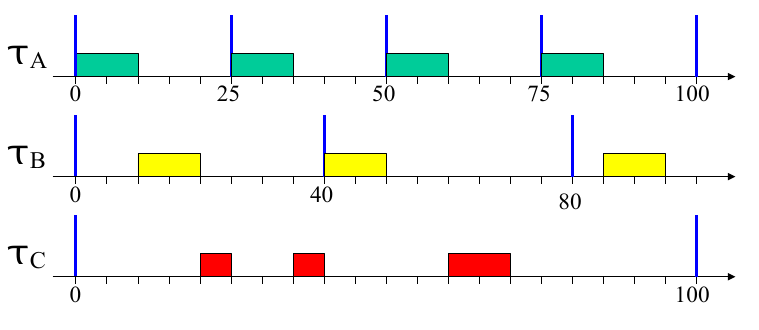
\includegraphics[width=0.5\textwidth]{img/rm_1}
\end{figure}
\\
Definiamo l'utilizzazione della \textit{CPU} da parte di un task come $U_i = \frac{C_i}{T_i}$, in questo modo possiamo andare a calcolare l'utilizzazione della \textit{CPU} su tutti i task definiti:
\begin{center}
    \[U_p = \sum_{i = 1}^{n} \frac{C_i}{T_i} \qquad \leftarrow U_p \text{ processor load} \]
\end{center}
In questo modo riusciamo a valutare il \textbf{carico del processore} che però \textbf{non} è una condizione \textbf{sufficiente} per garantire la \textbf{\textit{schedulabilità}} di un \textit{task set}, ma solo \textbf{necessaria}, infatti ci può dire se il \textit{task set} non è schedulabile in quanto $U_p > 1$ indica che il processore è \textit{overloaded}, ma nel caso in cui $U_p < 1$ ci possono essere dei casi in cui il \textit{task set} non può essere schedulato tramite \textit{RM}. \\
È possibile però identificare un punto, noto come $U_{lub}$ [\textit{least upper bound}] tale per cui sia possibile avere un \textbf{test di schedulabilità} sia \textbf{necessario} che \textbf{sufficiente}. Infatti nel caso in cui $U_p \leq U_{lub}$ il \textit{task set} è sicuramente schedulabile tramite \textit{RM}. Mentre nel caso in cui $U_{lub} < U_p \leq 1$ non possiamo dire niente di certo sulla fattibilità del \textit{task set}.
Per \textit{Rate Monotonic} $U_p^{RM} = n \cdot (2^{\frac{1}{n}} - 1)$ quindi avremo che: \[ \lim_{n\to\infty} U_{lub} = \log_2 2\]
Definiamo il \textbf{\textit{Critical Instant}} come l'istante di tempo in cui è presente il \textit{response time} maggiore, è stato dimostrato che equivale, considernado un \textit{task set} $\mathcal{T}$ all'istante in cui arrivano in corrispondenza tutti i task a più alta priorità. \\
Dal punto di vista della schedulabilità un task sporadico può essere considerato come un task periodico e quindi è possibile calcolarsi il suo $U_p$ e confrontarlo con l'$U_{lub}$ del \textit{task set}. \\
\textbf{\textit{Rate Monotonic}} è \textbf{ottimo}, infatti se esiste un assegnamento a priorità fisse che permette la fattibilità di uno \textit{schedule} per un \textit{task set} $\mathcal{T}$ allora l'assegnamento \textit{RM} è fattibile per il \textit{task set} $\mathcal{T}$, al contrario se un \textit{task set} non è schedulabile con \textit{RM} allora non esiste nessun altro assegnamento a priorità fissa che riesca a rendere fattibile la schedulazione del \textit{task set}. \\
\textbf{\textit{Hyperbolic Bound}}: \[ \prod_{i=1}^n (U_i + 1) \leq 2 \qquad \text{vs.} \qquad \sum_{i=1}^n U_i \leq n \cdot (2^{\frac{1}{n}} - 1)\]

\section{Earliest Deafline First}
Ogni \textit{job} riceve una \textit{deadline \textbf{assoluta}} $d_{i,k} = r_{i,k} + D_i$, in ogni istante di tempo il processore viene assegnato al \textit{job} con la \textit{earliest absolute deadline}, con EDF, qualsiasi set di attività può utilizzare il processore fino al 100\%.